\section{Introduction}

% \textbf{STYLE: Describe the problem, State your contributions - introduction makes claims >> The body of the paper provides evidence to support each claim}
% \textbf{STYLE: Use references here}

%  Application:  unmanned drones, intelligent glasses

% Terminology:
% Filter layer: convolutional kernel
% Output of layer: activation

% In general, the computational complexity of CNNs is dominated by the convolutional layers, while the number of parameters is mainly related to the fully connected layers

% Why is sparsity important: The high sparsity of the parameters after pruning introduces two benefits for deep neural networks. On the one hand, the sparse parameters after pruning require less disk storage since the parameters can be stored in the compressed sparse row format (CSR) or compressed sparse column (CSC) format. On the other hand, computations involving those pruned parameters are omitted; thus, the computational complexity of deep networks can be reduced.

% According to the granularity of the pruning, pruning methods can be categorized into five groups: (Figure 2 in recent advances in efficient computation
% fine-grained pruning, 
% vector-level pruning, 
% kernel level pruning, 
% group-level pruning
% filter-level pruning

% Pruning helps better generalization and of course model will require less number of training samples, 

% 1. Fine-grained tuning: 
% Good reference for early pruning [NIPS 1989, Yann LeCun], [1993, Babak Hassibi] using approximate second-order derivatives of the loss function w.r.t. the parameters  to determine the saliency of the parameters

%% APPLICATIONS and their PAPERS:
% From Edge-Host [Georgia-DAC]: example is a camera network with edge devices composed of an image sensor and a lightweight processor.
% From Edge-Host [Georgia-DAC] applications: This configuration is appealing in the applications where the host make central decision and control
% Vehicle detection and recognition: Yong Tang et al. Vehicle detection and recognition for intelligent traffic surveillance system.
% Remote monitoring: G. Chen et al. Deep convolutional neural network based species recognition for wild animal monitoring
% Scene analysis: Cong Zhang et al. Cross-scene crowd counting via deep convolutional neural networks. In CVPR, 2015.

% From Zeiler paper: (i) the availability of much larger training sets, with millions of labeled examples; (ii) powerful GPU implementations, making the training of very large models practical and (iii) better model regularization strategies, such as Dropout.

% From BranchyNet: Due to the computational costs of deep networks, improving the efficiency of feedforward inference has been heavily studied. Two such approaches are network compression and implementation optimization. Network compression schemes aim to reduce the the total number of model parameters of a deep network and thus reduce the amount of computation required to perform inference.

% From XNOR-NET: virtual reality and augmented reality

DNN architectures are promising solutions in achieving remarkable results in a wide range of machine learning applications, including, but not limited to computer vision, speech recognition, language modeling and autonomous cars. 

Currently, there is a major growing trend in introducing more advanced DNN architectures and employing them in end-user applications. The considerable improvements in DNNs are usually achieved by increasing complexity which requires more computational resources for training and inference. Recent research directions to make this progress sustainable are: development of Graphical Processing Units (GPUs) as the vital hardware component of both servers and mobile devices~\cite{GPU4NN}, design of efficient algorithms for large-scale distributed training~\cite{DistributedDNN} and efficient inference~\cite{SAMRAGH}, compression and approximation of models~\cite{efficientDNN}, and most recently introducing collaborative computation of cloud and fog as known as dew computing~\cite{DewComputing}. 

Using cloud servers for computation and storage is becoming extensively favorable due to technical advancements and improved accessibility. Scalability, low cost, and satisfactory Quality of Service (QoS), made offloading to cloud the typical choice for computing intensive tasks. On the other side, mobile-device are being equipped with more powerful general purpose CPUs and GPUs. Very recently there is a new trend in hardware companies to design dedicated chips to better tackle machine-learning tasks. For example, Apple's A11 Bionic chip~\cite{iPhoneX} used in iPhone X uses a neural engine in its GPU to speed up DNN queries of applications such as face identification and facial motion capture~\cite{animoji}. 

There are currently two methods for DNN inference: mobile only and cloud only. In simple models, a mobile device is responsible for performing all of the computation. In case of complex models, the raw input data (image, video stream, voice, etc.) is uploaded and then computed on the cloud. The results of the task are later downloaded to the device. 

Besides the improvements of the mobiles devices mentioned earlier, the computational power of mobile devices are still considered significantly weaker than the cloud ones. Therefore, mobile-only approach can cause large inference latency and failure in meeting QoS. Moreover, embedded devices undergo major energy consumption constraints due to battery capacity limits. On the other hand, cloud-only suffers communication overhead for uploading the raw data and downloading the outputs. Moreover, slowdowns caused by service congestions, subscription costs, and network dependency should be considered as downsides of this approach. 

The superiority and persistent improvement of DNNs is heavily dependent on providing huge amount of training data. Typically, this data is collected from different resources and later fed into network for training. The final model can then be delivered to different devices for inference functions. However, there is a trend of appearance of applications requiring adaptive learning in online environments, such as self driving cars and security drones \cite{AdaptiveCar}\cite{EASI}. Model parameters in these smart devices are constantly being changed based on their continuous interaction with surroundings. Complexity of these architectures with extended number of parameters and current cloud-only methods for DNN training, implies a constant communication cost and burden of increased power consumption for mobile device. 

Automatic partitioning of computationally extensive tasks over the cloud for optimization of performance and energy consumption has been already well studied~\cite{CloneCloud}. Most recently, scalable distributed hierarchy structures between end-user device, edge, and cloud have been suggested~\cite{CloudEdgeDevice} which are specialized for DNN applications. However, exploiting the layer granularity of DNN architectures for run time partitioning has not been studied throughly yet. 



\begin{figure}[h]
\centering
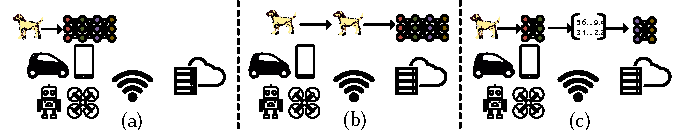
\includegraphics[width=\linewidth]{overall_system}
\caption{Different computation partitioning methods. (a) Mobile only: computation is completely done on mobile device. (b) Cloud only: raw input data is sent to cloud, computations is done on cloud and results are sent back to mobile device. (c) JointDNN: DNN architecture is partitioned at the granularity of layers, each layer can be computed either on cloud or mobile.}
\label{fig:fig_intro}
\end{figure}

% Story of the paper at the end of the introduction:
% Considering these char. we modeled it with a DAG
% Parameters of a DAG are
% Now you have a complete model, what do u want to solve, how do u want to solve it? Algorithm
% Parameters are extracted by experiments
% Results
% Conclusion
% Note: I did not mention the ILP for constraints! 
In this work, we are investigating inference and training of DNNs in a \textbf{joint} platform of mobile and cloud as an alternatives to the current single-platform methods as illustrated in Figure~\ref{fig:fig_intro}. Considering DNN architectures as an ordered sequence of layers, and possibility of computation of every layer either on mobile or cloud, we can model the DNN structure as a directed acyclic graph (DAG). The parameters of our real-time adaptive model are dependent on the following factors: mobile/cloud hardware and software resources, battery capacity, network specifications, and QoS. Based on this modeling, we show that the problem of finding the optimal computation schedule for different scenarios, i.e. best performance or energy consumption, can be reduced to the polynomial time shortest path problem. 

To present realistic results, we made experiments with real hardwares as mobile device and cloud. To model the communication between platform, we used different network technologies and the most recent reports on their specifications in the U.S. 

DNN architectures can be categorized based on functionality. These differences enforce specific type and order of layers in architecture, directly affecting the partitioning result in the collaborative method. For discriminative models, used in recognition applications, the layer size gradual decrease proceeding from input toward output~\ref{fig:DNN_category}. This sequence suggests computation of the first few layers on the mobile device to avoid excessive communication cost of uploading large raw input data. On the other hand, growth of the layer size from input to output in generative models used for synthesizing new data, implies the possibility of uploading small input to the cloud and later downloading and computing the last layers on the mobile device for better efficiency. Interesting mobile applications like image to image translation are implemented with autoencoder architectures, usually consisting of middle layers with smaller sizes compared to input and output. Consequently we expect the first and last layers to be computed on the mobile device in our collaborative approach. We examined eight well-known DNN benchmarks selected from these categories to illustrate their differences in collaborative computation approach. 

As we will see in Section~\ref{Results}, the communication between the mobile and cloud is the main bottleneck for both performance and energy in the collaborative approach. We investigated the specific characteristics of CNN layer outputs and introduced a lossless compression method to reduce the communication costs. 

State-of-the-art work for collaborative computation of DNNs~\cite{Neurosurgeon} only considers one offloading point, assigning computation of its previous layers and next layers on the mobile and cloud platforms, respectively. We show that this approach is non-generic and fails to be optimal, and introduced a new method granting the possibility of computation on either platforms for each layer independent of other layers. Our evaluations show that JointDNN significantly improves the latency and energy up to $3\times$ and $7\times$ respectively compared to the status-quo single platform approaches without any compression. The main contributions of this paper can be listed as:

\begin{itemize}
\item Introducing a novel model for collaborative computation between the mobile and cloud 
\item Formulating the problem of optimal computation scheduling of DNNs at layer granularity in mobile cloud computing environment as shortest path problem and integer linear programming (ILP) 
\item Examining compressibility of DNN layers and developing a lossless compression method to improve communication costs
\item Demonstrating the significant improvements of performance, mobile energy consumption, and cloud workload achieved by using \textbf{JointDNN}
\end{itemize}

\begin{figure}
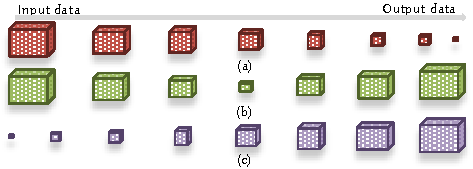
\includegraphics{architectures_layer_size}
\caption{Typical layer size architecture of (a) Discriminative (b) Autoencoder (c) Generative models.}
\label{fig:DNN_category}
\end{figure}

